\documentclass[12pt,letterpaper]{article}
\usepackage[utf8x]{inputenc}
\usepackage{ucs}
\usepackage[spanish]{babel}
\usepackage{amsmath}
\usepackage{amsfonts}
\usepackage{amssymb}
\usepackage{graphicx}
\usepackage{apacite}
\usepackage[left=2cm,right=4cm,top=2cm,bottom=2cm]{geometry}
\author{Sergio de Jesús Hernández Sánchez; Brando Martín Rivero Pérez}
\pretolerance=2000
\tolerance=3000

\begin{document}
	\begin{titlepage}
		\pagestyle{empty}
		\centering
		
\includegraphics[scale=.25]{IMAGENES/LOGO_UAEMEX.png}\\
		{\bfseries\LARGE Universidad Autonoma del Estado de Mexico\par}
		\vspace{1cm}
		{\bfseries\LARGE C.U Texcoco\par}
		\vspace{1cm}
		{\scshape\Large Ingeniería en Computación \par}
		\vspace{3cm}
		{\scshape\Huge Protocolo de tesis\par}
		\vspace{3cm}
		{\itshape\Large Algoritmos Geneticos para la seleccion automatica de caracteristicas en la deteccion de retinopatia por medio del tratamiento de imagenes  \par}
		\vfill
		{\Large Alumno: \par}
		{\Large Brando Martin Rivero Perez\par}
		\vfill
		{\Large Noviembre 2021 \par}
	\end{titlepage}
	\newpage
	\pagestyle{empty}
	\tableofcontents
	\listoffigures
	\listoftables
	\newpage
	\setcounter{page}{1}
	\pagestyle{plain}
	

\section{Introducción}

\bigskip

La diabetes es considerado un problema de saludo a escala global, y es considerada una de las enfermedades mas complejas, caracterizada principalmente por la falta de la secreción de  insulina por parte del páncreas, así mismo como por la resistencia del cuerpo a la insulina.


Las personas que viven con diabetes mellitus constantemente están preocupados por su estado de salud, este trabajo de investigación se realiza con el objetivo de presentar una herramienta medica para así poder brindarle a esas personas una mayor seguridad en cuanto salud visual, para esto buscamos hacer uso de programas digitales e inteligencia artificial, así como algoritmos genéticos desarrollados con este fin.\cite{Esparza}

En México la diabetes mellitus es la primer causa de muerte en mujeres y la segunda en hombres, esta puede provocar complicaciones a largo plazo, siendo la retinopatía y el gloucoma parte de estas, por lo cual la pronta detección de estas puede ayudar a que muchas personas lleven el tratamiento clínico necesario y así evitar la perdida total de visión como en muchos casos.

La retinopatía diabética fue descrita por primera vez 
hace mas de 100 años por MacKenzie (1879) y por Nettleship (1888) Con el uso generalizado de la insulina y el aumento sustancial de la supervivencia de las personas con diabetes, las complicaciones tardías de la enfermedad se volvieron cada vez más prominentes.
La retinopatía diabética es la causa más frecuente de nuevos casos de ceguera entre los adultos de 20 a 74 años.\cite{Dosal}

La retinopatía diabética es la principal causa de perdida visual no recuperable en los países industrializados, prevaleciendo en pacientes entre los 20 y 64 años de edad, siendo responsable de 10\% de nuevos casos de ceguera cada año.\cite{Aliseda} 
 
Según el Dr. Arturo Hernandez Piña, medico oftalmológico del Centro de investigación en diabetes, obesidad y nutrición (CIDON) \"\ Uno de cada cuatro casos de ceguera se presentan que se presentan en nuestro medio tiene su origen en esta complicación de la diabetes\"\ haciendo referencia a la retinopatía diabética.

Es importante realizar estudios constantes a pacientes con diabetes para poder determinar las complicaciones a tiempo, existen diversos exámenes para la detección de la retinopatía; la retinografia y el examen de fondo de ojo con pupila dilatada en consulta oftalmológica, siendo la retinografia, la captura fotográfica del fondo del ojo, mientras que el examen de fondo de ojo con pupila dilatada requiere la dilatación provocada de la pupila para poder realizar el estudio, permaneciendo la pupila dilatada y visión borrosa por horas. La tomografía láser de barrido son costosas y accesibles solo en centros oftálmicos especializados. \cite{Stapor2004}


El desarrollo de sistemas de algoritmos genéticos han ayudado a resolver problemas en los cuales son necesarios el estudio de muchos sujetos.\cite{Merino2019} En los últimos años este tipo de estudios han tenido un desarrollo amplio ya que es una opción para resolver problemas de la vida real.
Los algoritmos genéticos son inspirados por el comportamiento evolutivo de los genes en los seres vivos, estos se apoyan de la inteligencia artificial ya que se necesita un sistema que simule el comportamiento de los seres vivos.\cite{Diagnosis4799}


\newpage
\begin{center}
	\section{Problemática}
	\hrule
\end{center}
Datos otorgados por la Asociacion Mexicana de Retina indican que en Mexico hay un aproximado de 2 millones de pacientes diagnotiscados con Retinopatia dibatica, mientras que mas de trecientos mil padecen de un grado avanzado de con un riesgo muy elevado de que evolucione a ceguera.

El gobierno de Mexico indica que este padecimiento cronico y progresivo tiene una prevalencia de 31.5\% en Mexico.

La Universidad Nacional Autonoma de Mexico indica que en Mexico hay un aproximado de 12 millones de personas con diabetes.

Actualmente México es uno de los países con mayor ocurrencia de casos de diabetes en el mundo. En 1995 ocupaba el noveno lugar con mayor número de casos de diabetes y se espera que para el año 2030 ocupe el séptimo\cite{Mexico.Estudio2011}. En México la diabetes es de las principales causas de mortalidad y con el transcurso de los años muestra un incremento progresivo.\cite{CarmenDubonPeniche2010}
\\
\newpage
\begin{center}
	\section{Justificación}
	\hrule
\end{center}

Los exámenes para la detección de la retinopatía han avanzado, pero algunos siguen siendo dolorosos o molestos para quienes los utilizan, con una probabilidad de que el resultado falle y haya la necesidad de realizar el examen de nuevo.

En la retina existen 2 condiciones causantes de disminución de la agudeza visual: el edema macular diabético y la neovascularización retinal (crecimiento anormal de vasos sanguíneos).\cite{Diagnosis4799} Se ha demostrado claramente que por lo menos 4-5 años de la enfermedad debe transcurrir antes de las primeras lesiones (Microaneurismas capilares y hemorragias en punto) Entre el 5to a 10mo año del inicio de la DM la prevalencia de RD se incrementa.\cite{Merino2019}


Durante las etapas iniciales la retinopatía diabética  suele no presentar síntomas.
\\
\newpage

\section{Objetivos}


\subsection{Objetivo General}


El objetivo general de este trabajo de investigación es realizar un algoritmo capaz de seleccionar las características texturales principales para la detección temprana de Glaucomas en pacientes diagnosticados con diabetes.
\\
\subsection{Objetivos Específicos}
\begin{itemize}
	\item Definir las caracteristicas que son requeridas.
	\item Segmentar por características de color utilizando algoritmos geneticos.
	\item Probar el funcionamiento del algoritmo.
	\item Discutir resultados y conclusiones obtenidas.
\end{itemize}
\newpage
\section{Metodologia}

\begin{enumerate}
	\item Adquirir el  objeto para realizar la dereccion
	\item Digitalizar, cuantilizar, comprender y limitar el objeto
	\item Segmentar
	\item Seleccionar las caracteristicas
	\item Realizar la representacion de los datos para ser procesados
	\item Interpretar el resultado
\end{enumerate}

\section{Metas y entregables}
\begin{itemize}
	\item Librerias de los algoritmos genenticos de seleccion de caracteristicas programado en matlab
	\item Tesis
\end{itemize}
\section{Cronograma}
	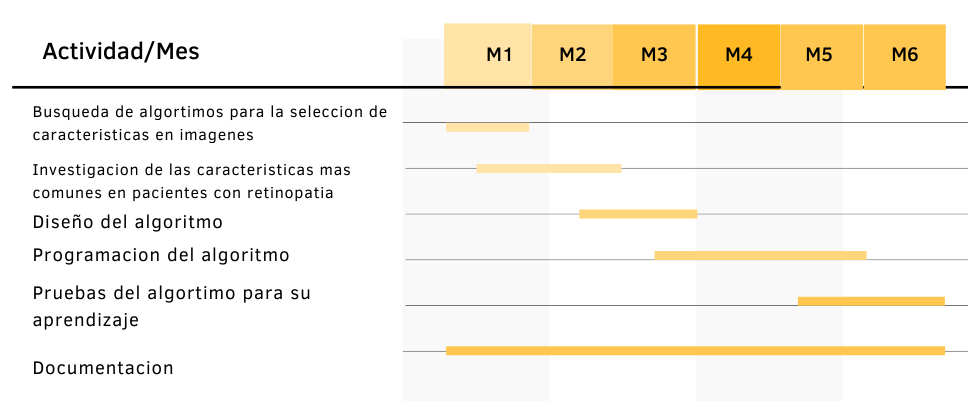
\includegraphics[scale=.5]{IMAGENES/ActividadMes.png}
\newpage
\bibliographystyle{apacite}
\bibliography{Referencias}



\newpage


\end{document}